\chapter{Preprocessing}
\label{chap:preprocessing}

With a clean set of 21 recordings and 93 aligned seizures in hand, the next step was to turn
continuous EEG into something a classical machine-learning model can actually consume: short,
fixed-length windows, each described by a fixed set of numbers. This chapter covers the filter,
the windowing, and the feature extraction, in that order --- and explains why each choice was
made, not just what it was.

\section{The frequency filter}

Every recording is passed through a 4th-order Butterworth band-pass filter, 0.5--40~Hz, applied
\emph{zero-phase} --- forward and then backward through the signal, not a single forward pass.

Three separate decisions sit inside that one filter, each for its own reason.

\begin{itemize}[leftmargin=1.4em]
  \item \textbf{0.5~Hz low cutoff.} Strips slow baseline drift --- sweat, skin-potential drift,
    slow head movement --- without touching the frequency range where seizure activity and
    normal brain rhythms actually live.
  \item \textbf{40~Hz high cutoff.} Removes high-frequency muscle and movement noise, and sits
    safely below 50~Hz mains hum (the local electrical mains frequency), so that hum is
    attenuated along with everything else above 40~Hz.
  \item \textbf{Zero-phase filtering.} A normal, single-pass (causal) filter introduces a time
    lag. Filtering forward and backward cancels that lag out, so a filtered seizure's boundaries
    land on exactly the same timestamps as the original annotated boundaries. This matters
    because the entire evaluation later in this report depends on precise event timing.
\end{itemize}

\begin{figure}[H]
  \centering
  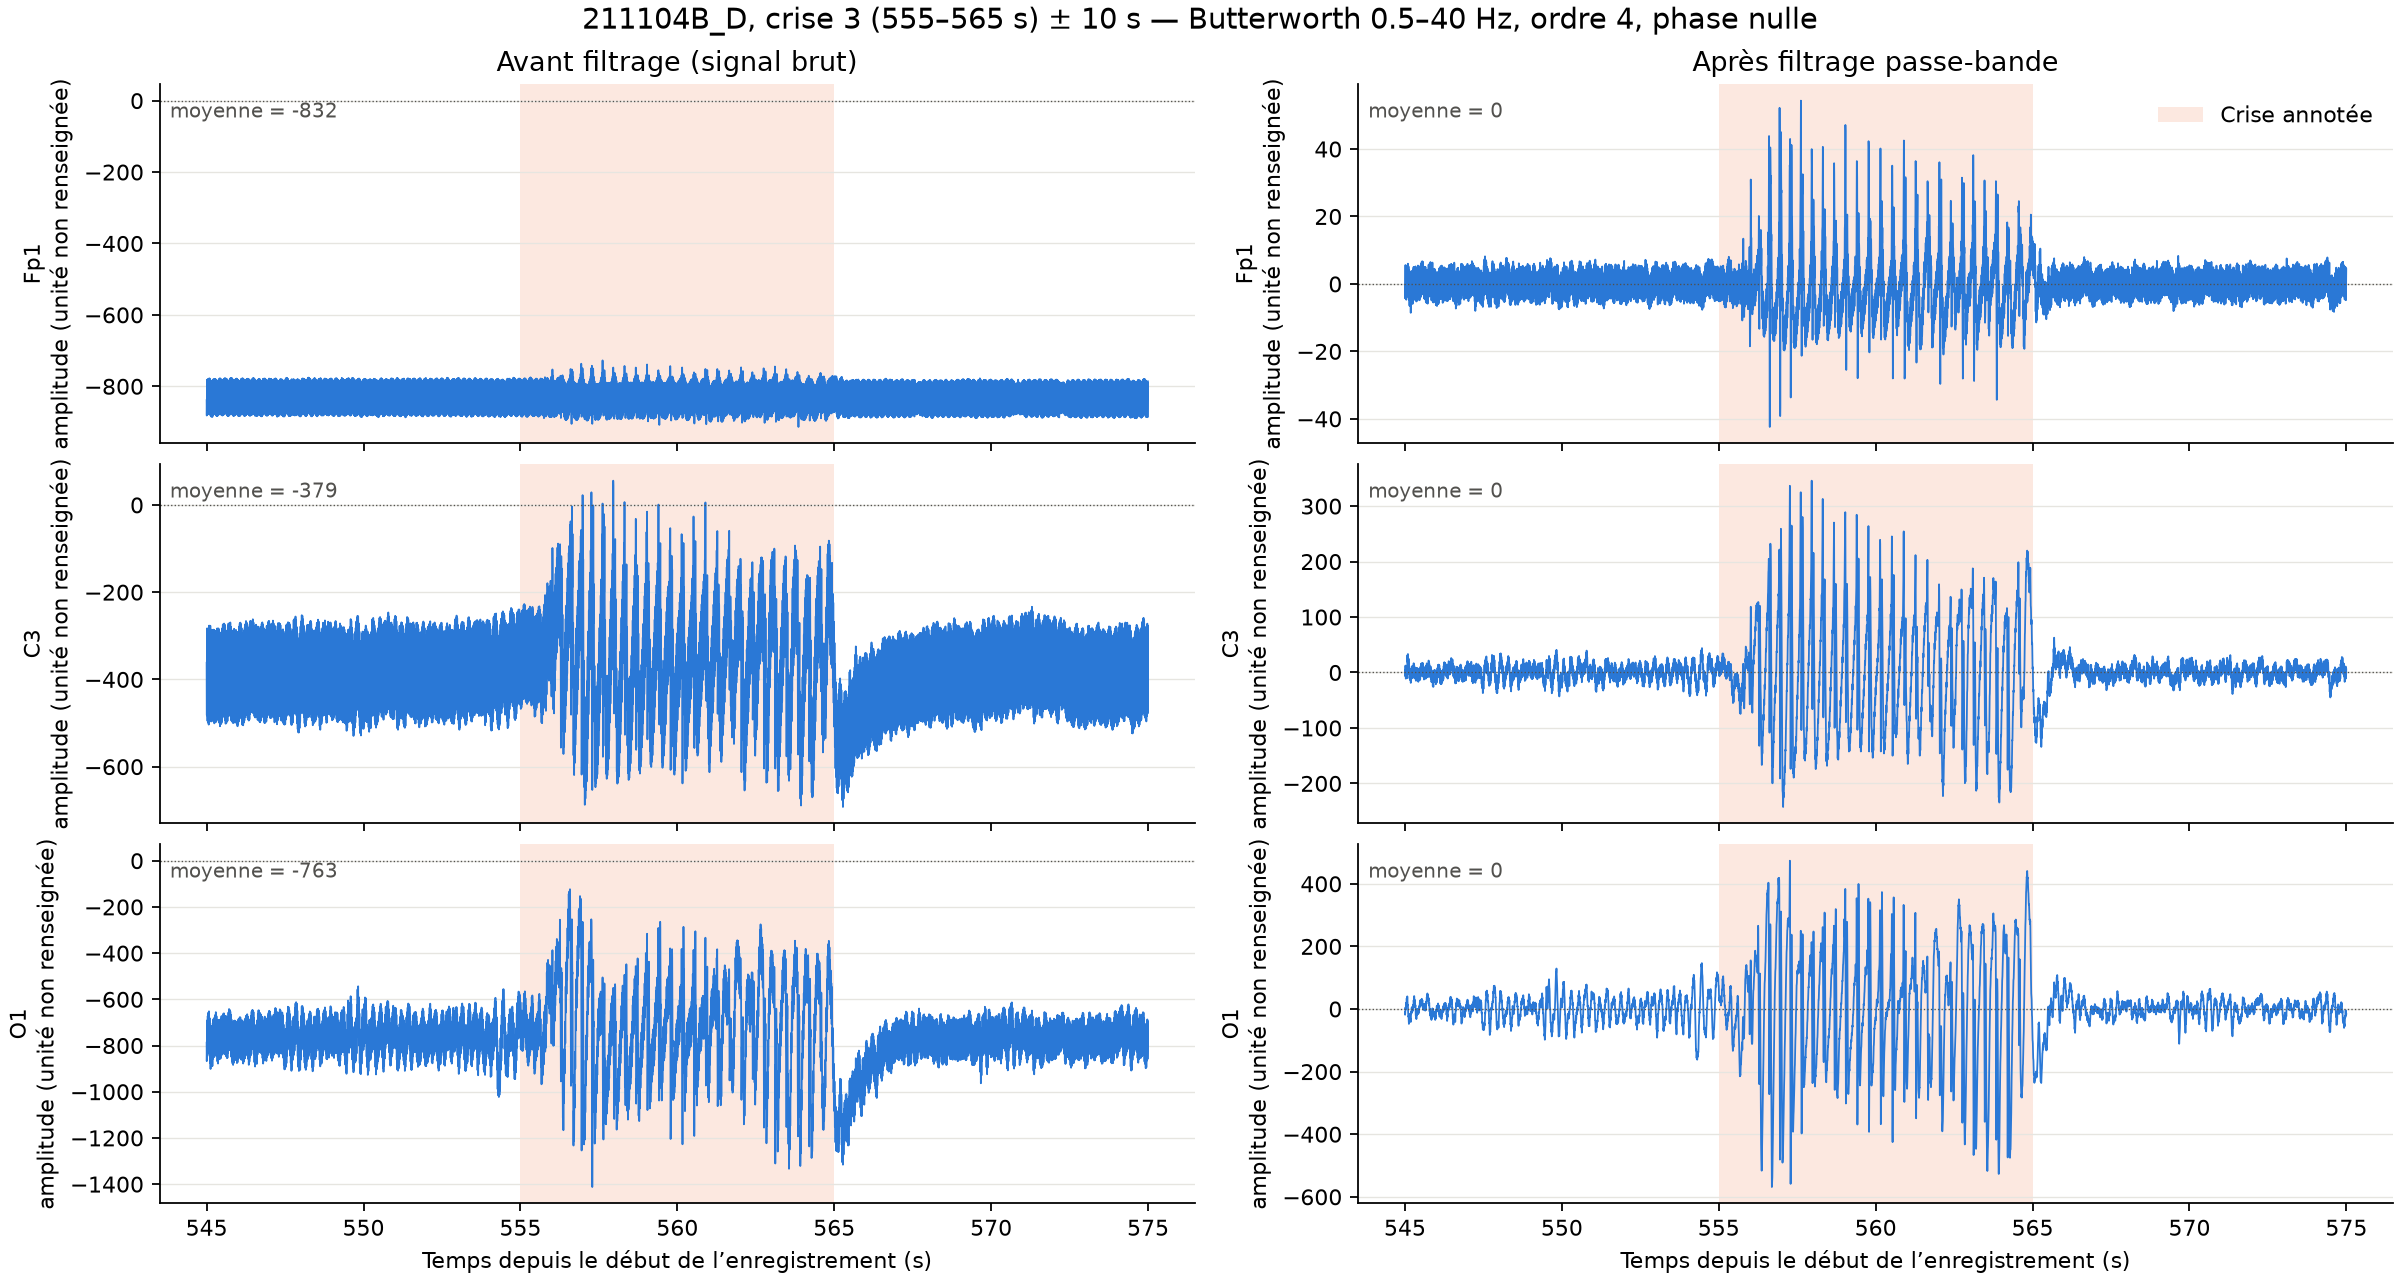
\includegraphics[width=0.9\linewidth]{official/preprocessing/211104B_D_seizure3_filtering.png}
  \caption{A real seizure segment from \texttt{211104B\_D} before and after the 0.5--40~Hz
    zero-phase band-pass filter.}
  \label{fig:filtering-example}
\end{figure}

\section{Windowing}

The filtered signal is cut into 2-second windows with 50\% overlap between consecutive windows.
A window is labeled as a seizure window (class 1) if at least half of its samples fall inside an
annotated seizure; otherwise it is labeled class 0.

This produces 31{,}419 windows in total: 1{,}244 of them seizure windows (3.96\%), and
30{,}175 non-seizure (96.04\%). Fewer than four windows in a hundred contain a seizure. This
imbalance is built into the problem itself by the rarity of the events being detected --- it is
not an artifact of this particular split, and it shapes every modeling decision in
\Cref{chap:classicalml,chap:augmentation}.

\section{Feature extraction}

Each 2-second window is reduced to 320 numbers before it reaches a classical model. These are
not learned; they are hand-designed, computed directly from the filtered signal.

\textbf{Why features, and not the raw signal, for the classical pipeline:} classical models such
as a decision tree or an SVM need a fixed-length input vector to begin with, and with only 93
seizures in the entire dataset, hand-crafted features generalize far better than asking a model
to discover its own representation from 512 raw samples per channel. (The deep-learning
comparison in \Cref{chap:deeplearning} takes the opposite approach, learning directly from raw
signal, precisely so the two approaches can be compared.)

\subsection{Sixteen feature types, twenty columns each}

There are 8 time-domain feature types, computed per channel over each window: mean, standard
deviation, variance, minimum, maximum, peak-to-peak amplitude, root-mean-square, and energy
(the sum of squared samples).

There are 8 frequency-domain feature types, built from 4 frequency bands --- delta
(0.5--4~Hz), theta (4--8~Hz), alpha (8--13~Hz), and beta (13--30~Hz) --- each contributing an
absolute band-power feature and a relative band-power feature (absolute power divided by the
total power across 0.5--30~Hz). Band power is computed from a Hann-windowed power spectral
density of each window.

\[
  \underbrace{8~\text{time-domain}}_{\text{mean, std, var, min, max, amplitude, rms, energy}}
  +
  \underbrace{8~\text{frequency-domain}}_{\text{4 bands} \times \text{absolute \& relative power}}
  = 16~\text{feature types}
\]

Each of these 16 feature types is computed separately for every one of the 19 EEG channels, plus
one additional column averaging that feature across all 19 channels --- 20 columns per feature
type.

\[
  16~\text{feature types} \times 20~\text{columns (19 channels + 1 average)} = 320~\text{features}
\]

This is the exact arithmetic behind the ``320 features'' figure quoted throughout this project.

\subsection{Which channels end up mattering}

Once a Random Forest is trained on these 320 features (\Cref{chap:classicalml}), it is possible
to ask which channels it actually relies on, by reading off scikit-learn's built-in feature
importance and grouping it by channel.

\begin{figure}[H]
  \centering
  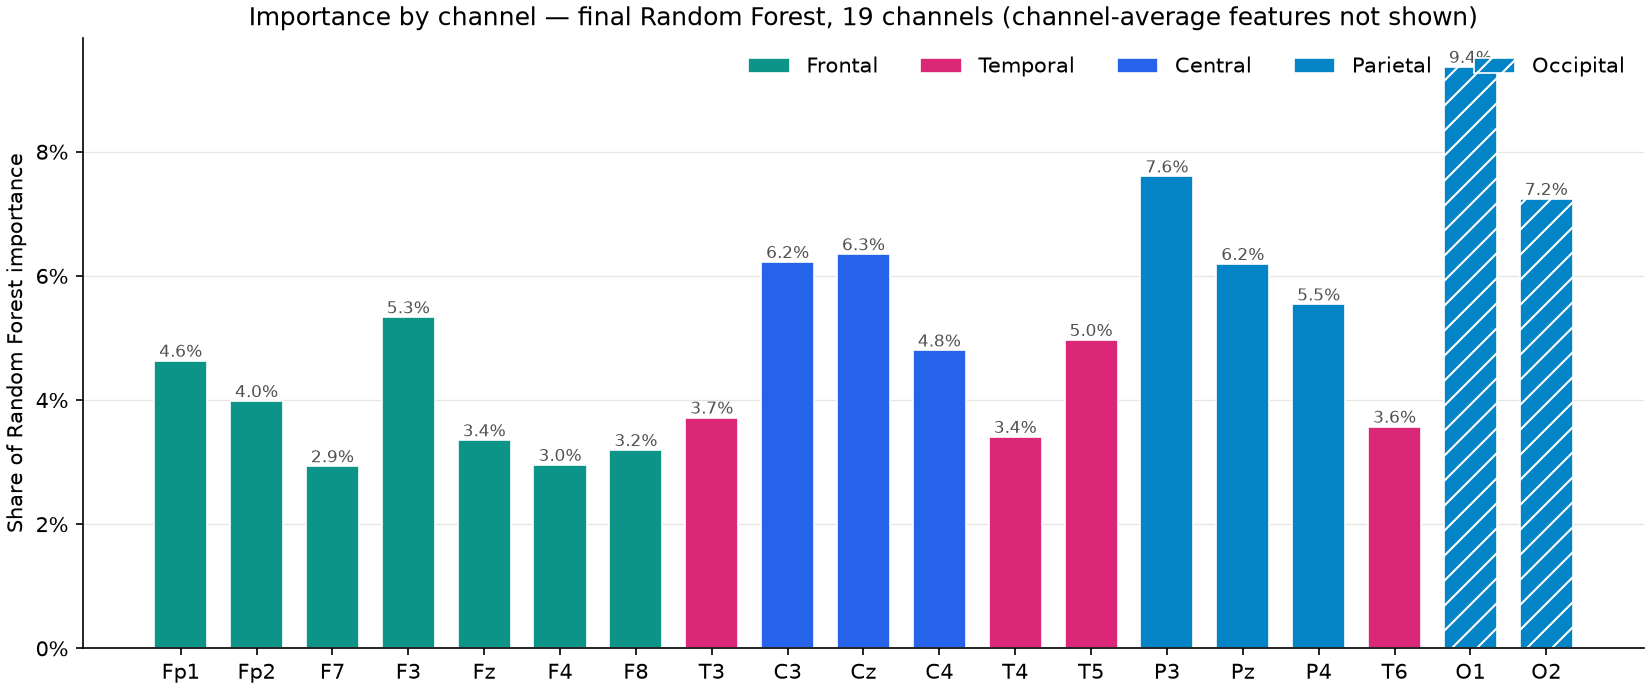
\includegraphics[width=0.95\linewidth]{official/channels/importance_by_channel.png}
  \caption{Random Forest feature importance, summed per channel (the cross-channel average
    columns are excluded here, to show per-channel differences clearly).}
  \label{fig:channel-importance}
\end{figure}

The occipital channels, O1 and O2, carry noticeably more importance than any other single
channel (9.4\% and 7.2\% of the total, respectively), with the parietal channels P3 and Pz
close behind. The frontal channels, by contrast, carry the least importance individually,
despite there being more of them. No channel dominates outright --- the heaviest single channel
still accounts for under 10\% of the total importance --- which is consistent with absence
seizures being a generalized, whole-scalp pattern rather than one localized to a single
electrode.

\begin{summarybox}
A 4th-order, zero-phase Butterworth band-pass filter (0.5--40~Hz) cleans drift and mains hum
without shifting seizure timing. The cleaned signal is cut into 31{,}419 windows of 2 seconds
with 50\% overlap, of which only 1{,}244 (3.96\%) contain a seizure --- the central imbalance
problem the rest of the classical pipeline has to deal with. Each window is reduced to 320
hand-crafted features: 8 time-domain and 8 frequency-domain feature types, each computed across
19 channels plus a cross-channel average.
\end{summarybox}
